\subsubsection{09.04.15}
\begin{enumerate}
	
	\item The time of beginning and ending of the meeting: 1:00 - 2:00.
	
	\item Purposes of the meeting: 
	\begin{enumerate}
		
		\item To understand how to work with the chain.
		
		\item To start assemble new wheel base.
		
	\end{enumerate}
	
	\item Work that has been done:
	\begin{enumerate}
		
		\item Today we understood how to use the instrument for unlocking the chain and how to connect it by this instrument.
		
		\item There were installed 4 motors with gears and sprockets for chain which were fixed by two couplers. So there is a very small probability that they will get off during the match.
		\begin{figure}[H]
			\begin{minipage}[h]{0.2\linewidth}
				\center  
			\end{minipage}
			\begin{minipage}[h]{0.6\linewidth}
				\center{
\includegraphics[scale=0.3]{days/09.04.15/images/01}}
				\caption{We began assembling the wheelbase}
			\end{minipage}
		\end{figure}
		
		\item From the left side we held the chain between the motors and axis with front wheel. Firstly we located it so that it hooked the floor. But when we found it we turned motors in their mounts and this problem disappeared.
		
		\item We installed one mount for additional motor that will rotate wheel.
		\begin{figure}[H]
			\begin{minipage}[h]{0.2\linewidth}
				\center  
			\end{minipage}
			\begin{minipage}[h]{0.6\linewidth}
				\center{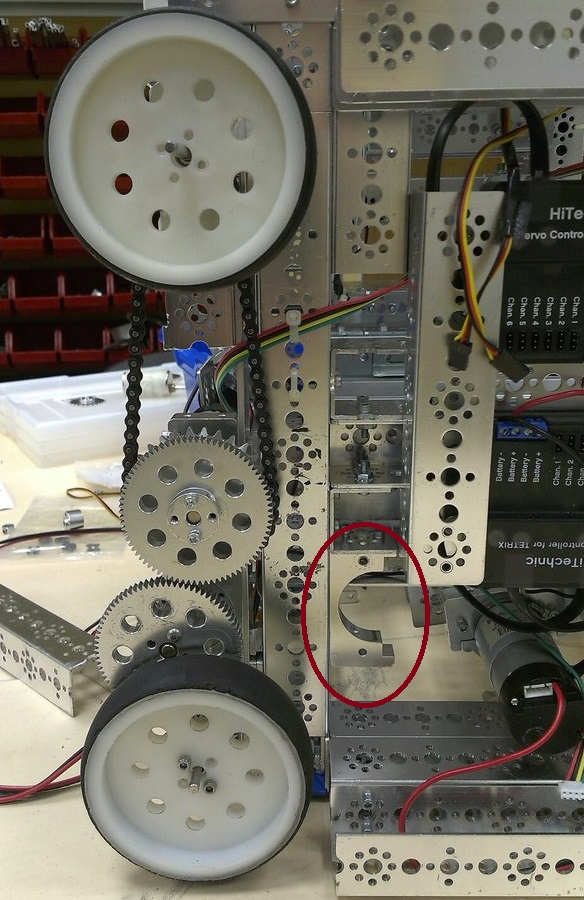
\includegraphics[scale=0.24]{days/09.04.15/images/02}}
				\caption{Mount for the 3-rd motor}
			\end{minipage}
		\end{figure}
		
	\end{enumerate}
	
	\item Results:
	\begin{enumerate}
		
		\item We understood how to work with the chain.
		
		\item Wheel base partially assembled.
		
	\end{enumerate}
	
	\item Tasks for the next meetings:
	\begin{enumerate}
		
		\item To finish wheel base.
		
		\item To buy fishing cord and use it for mount for blocks.
		
	\end{enumerate}
\end{enumerate}
\fillpage
